\section{Auswertung}
\label{s:Auswertung}

\subsection{Fehlerrechnung}
\label{sec:Fehlerrechnung}
Für die Fehlerrechnung werden folgende Formeln aus der Vorlesung verwendet.
für den Mittelwert gilt
\begin{equation}
    \overline{x}=\frac{1}{N}\sum_{i=1}^N x_i ß\; \;\text{mit der Anzahl N und den Messwerten x} 
    \label{eqn:Mittelwert}
\end{equation}
Der Fehler für den Mittelwert lässt sich gemäß
\begin{equation}
    \increment \overline{x}=\frac{1}{\sqrt{N}}\sqrt{\frac{1}{N-1}\sum_{i=1}^N(x_i-\overline{x})^2}
    \label{eqn:FehlerMittelwert}
\end{equation}
berechnen.
Wenn im weiteren Verlauf der Berechnung mit der fehlerhaften Größe gerechnet wird, kann der Fehler der folgenden Größe
mittels Gaußscher Fehlerfortpflanzung berechnet werden. Die Formel hierfür ist
\begin{equation}
    \increment f= \sqrt{\sum_{i=1}^N\left(\frac{\partial f}{\partial x_i}\right)^2\cdot(\increment x_i)^2}.
    \label{eqn:GaussMittelwert}
\end{equation}
\subsection{Bestimmung der Schallgeschwindigkeit und der Dicke der Anpassungsschicht}
Die Abmessungen der einzelnen Bohrungen befinden sich in \autoref{tab:block}. Die Nummerierung der Bohrungen befinden sich in \autoref{fig:acryl}.
\begin{table}
    \centering 
    \caption{Abmessungen der einzelnen Bohrungen}
\begin{tabular}{c c c c}
    \toprule
    Bohrung & Abstand von unten in \unit{\mm} & Abstand von oben \unit{\mm} & Durchmesser d in \unit{\mm}\\
    \midrule
    1&59.0&19.2&1.7 \\
     2&60.7&17.5&1.7 \\
     3&13.2&60.6&6.0 \\
     4&21.7&53.2&5.0 \\
     5&30.0&45.6&4.0 \\
     6&38.6&38.0&3.0 \\
     7&46.6&29.8&3.0 \\
     8&54.7&22.8&3.0 \\
     9&62.7&13.7&3.0 \\
     10&70.7&6.8&3.0 \\
    11&15.3&54.4&9.9 \\
    \bottomrule
    \end{tabular}
    \label{tab:block}
\end{table}

Um die Schallgeschwindigkeit und die Dicke der Anpassungsschicht zu bestimmen, werden für sieben Bohrungen die Laufzeiten bestimmt. Diese befinden 
sich in \autoref{tab:geschw}.

\begin{table}
    \centering 
    \caption{Messwerte der Laufzeiten der einzelnen Bohrungen}
\begin{tabular}{c c}
    \toprule
    Bohrung & Laufzeit $t$ in \unit{\micro\s}\\
    \midrule
    3&45.4 \\
      4&39.9 \\
      5&34.4 \\
      6&29.0 \\
      7&23.0 \\
      8&17.1 \\
      9&11.1 \\
      \bottomrule
    \end{tabular}
    \label{tab:geschw}
\end{table}

Nun werden die Abstände der Bohrungen von der oberen Fläche gegen die Hälfte der Laufzeiten aufgetragen (da die Strecke bis zum Loch zweimal 
durchlaufen wird) und eine Ausgleichsgerade gebildet. Diese befinden sich in \autoref{fig:plotv}.
\begin{figure}
    \centering
    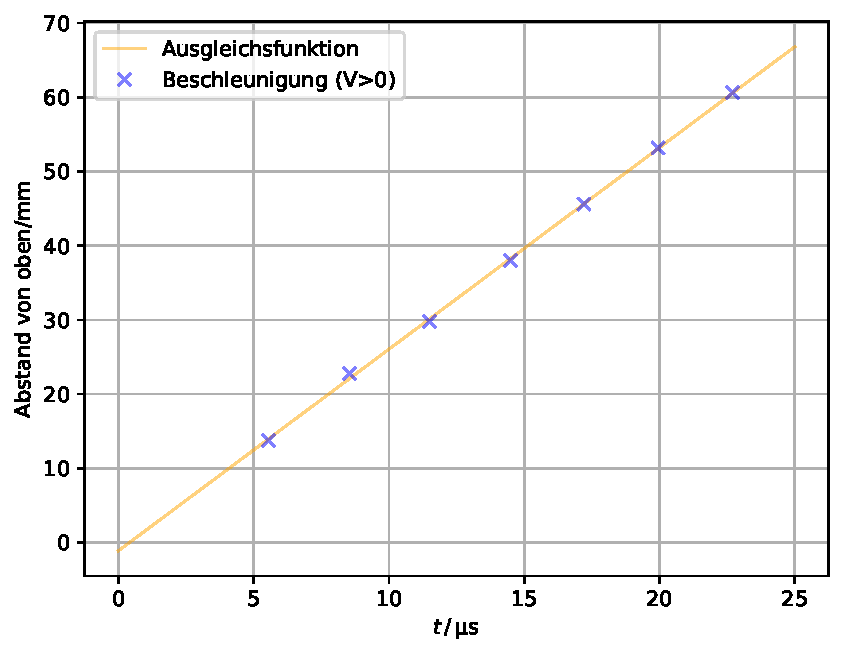
\includegraphics[height = 8cm]{build/plotv.pdf}
    \caption{Regression zur Bestimmung der Schallgeschwindigkeit und der Dicke der Anpassungsschicht.}
    \label{fig:plotv}
\end{figure}

Die Schichtdicke entspricht dem Betrag des y-Achsenabschnitt
\begin{equation*}
    d = \lvert b\rvert = \lvert (-1.1 \pm 0.4) \, \unit{\mm}\rvert =  (1.1 \pm 0.4) \, \unit{\mm} \; .
\end{equation*}
Die Schallgeschwindigkeit in Acryl ergibt sich über die Steigung der Ausgleichsgeraden
\begin{equation*}
    v = (2.718 \pm 0.025) \, \unit{\mm \per \micro\s} = (2718\pm 25) \, \unit{\m\per\s} \; .
\end{equation*}

\subsection{Untersuchung des Acrylblocks mit einem A-Scan}
Die Messwerte des A-Scans von der oberen und unteren Seite des Acrylblocks befinden sich in \autoref{tab:AScan}. Dabei wurden die Tiefenmessungen 
mit der Schichtdicke korrigiert. Mithilfe der korrigierten Werte und der gemessenen Gesamthöhe des Blocks $h = 79.9\,\unit{\mm}$ ergibt sich über 
\begin{equation*}
    d = h - a_{\symup{ob}} - a_{\symup{unt}}
\end{equation*}
der Durchmesser der einzelnen Bohrungen, welcher ebenfalls in \autoref{tab:AScan} dargestellt ist.

\begin{table}
    \centering 
    \caption{Messwerte der Tiefe der einzelnen Bohrungen sowie dessen Durchmesser.}
\begin{tabular}{c | c c | c c | c}
    \toprule
    & \multicolumn{2}{c}{oben}& \multicolumn{2}{c}{unten} & \\
    Bohrung & Tiefe \/\unit{\mm} &  nach Korrektur \/\unit{\mm}& Tiefe \/ \unit{\mm} & nach Korrektur \/ \unit{\mm} & d \/ \unit{\mm}\\
    \midrule
                        1&20.6&19.5&60.4&59.3&1.1 \\
                         2&19.0&17.9&62.0&60.9&1.1 \\
                         3&62.0&60.9&14.5&13.4&5.6 \\
                         4&54.5&53.4&23.0&21.9&4.6 \\
                         5&46.9&45.8&31.6&30.5&3.6 \\
                         6&39.5&38.4&40.1&39.0&2.5 \\
                         7&31.4&30.3&47.9&46.8&2.8 \\
                         8&23.3&22.2&56.0&54.9&2.8 \\
                         9&15.2&14.1&64.1&63.0&2.8 \\
                        10&7.2&6.1&--&--& \\
                        11&55.8&54.7&16.8&15.7&9.5 \\
                        \bottomrule
    \end{tabular}
    \label{tab:AScan}
\end{table}

Die zehnte Bohrung konnte von unten nicht gemessen werden, da die elfte Bohrung direkt davor liegt und nicht genug Ultraschallwellen zu der zehnten Bohrung 
transmittiert werden, sodass diese messbar wäre.

\subsection{Untersuchung des Auflösungsvermögens}
Hier wurden die Bohrungen eins und zwei mit einem A-Scan untersucht. Dabei werden die Untersuchungen mit einer 1-MHz-Sonde und einer 2-MHz-Sonde miteinander
verglichen. Die Graphik der 1-MHz-Sonde befindet sich in \autoref{fig:1son} und die der 2-MHz-Sonde in \autoref{fig:2son}.

\begin{figure}
    \centering
    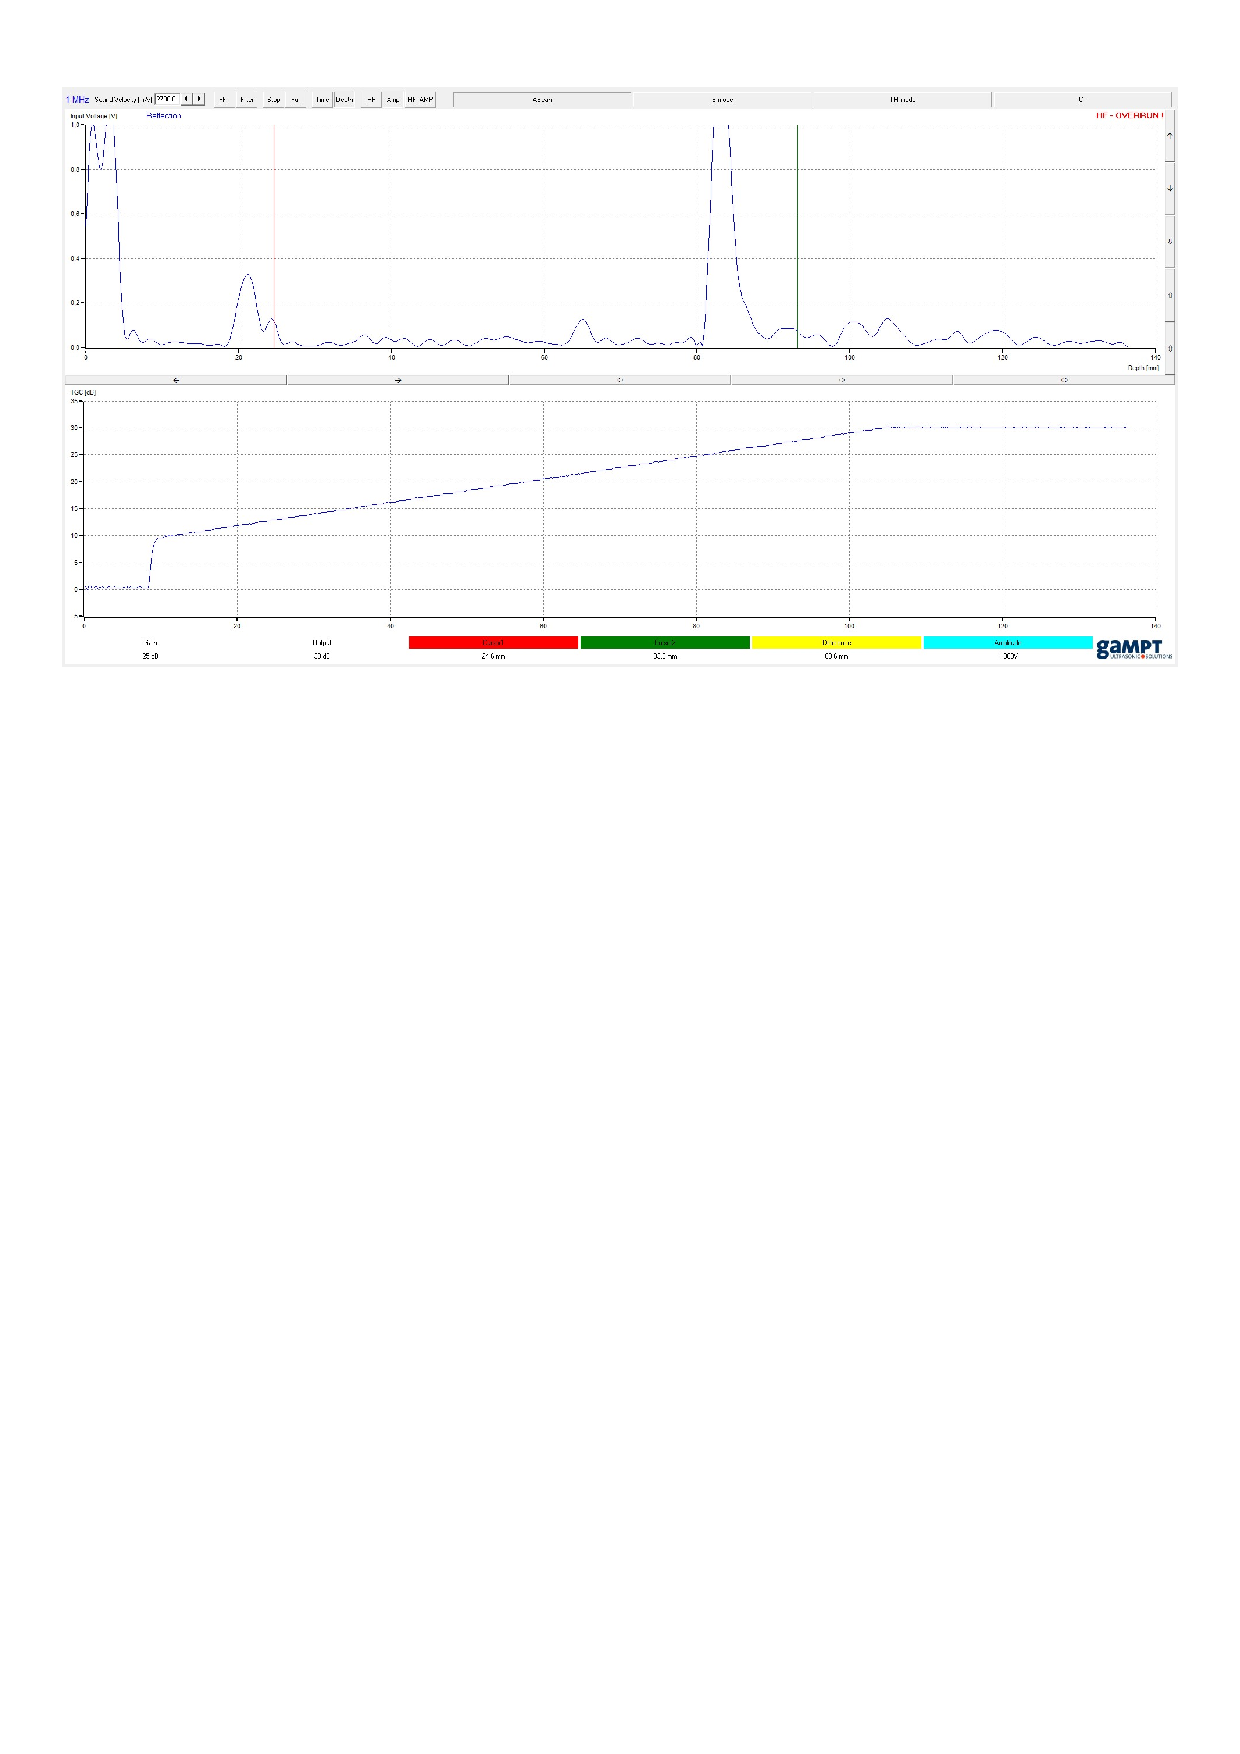
\includegraphics[height = 4cm]{1MHz.pdf}
    \caption{Graphik der 1-MHz-Sonde.}
    \label{fig:1son}
\end{figure}

\begin{figure}
    \centering
    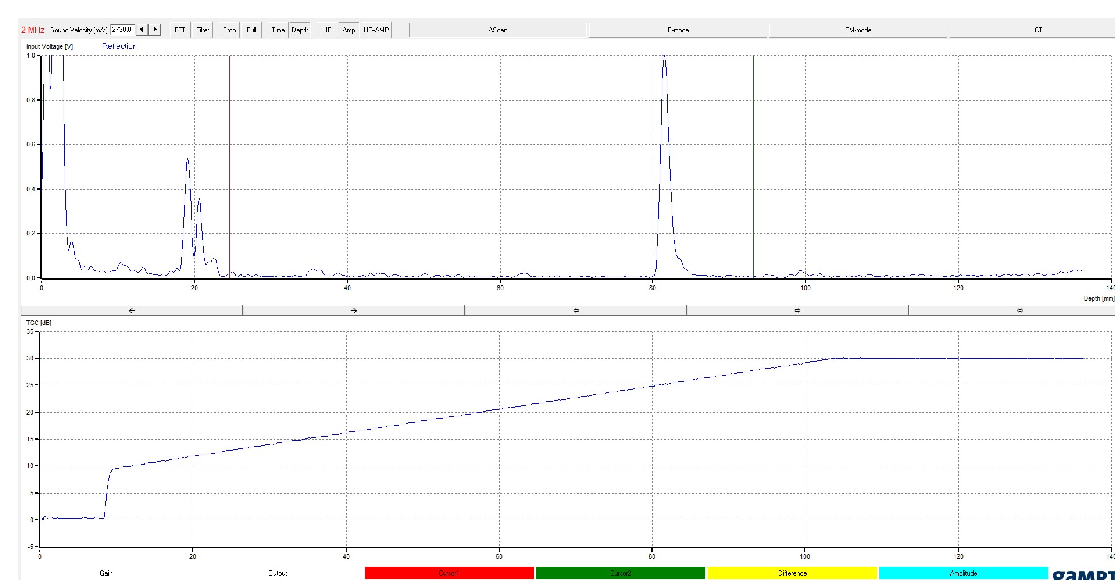
\includegraphics[height = 4cm]{2Mhz.pdf}
    \caption{Graphik der 2-MHz-Sonde.}
    \label{fig:2son}
\end{figure}

Wenn die beiden Peaks ungefähr auf der Höhe von $20\,\unit{\mm}$ der beiden Graphiken miteinander verglichen werden, wird festgestellt, dass die 2-MHz-Sonde 
ein höheres Auflösungsvermögen hat. Dies erkennt man daran, dass die Peaks bei der 1-MHz-Sonde undeutlich und schwieriger abzulesen sind.

\subsection{Untersuchung des Acrylblocks mit einem B-Scan}
\label{Sec:AuswertungBScan}
Um die Tiefen der Störstellen zu bestimmen, wurde im Programm der Ort der jeweiligen Stelle abgelesen und notiert. Die Berechnung
des Durchmessers erfolgt analog zu jener des A-Scans. 
\begin{figure}
    \centering
    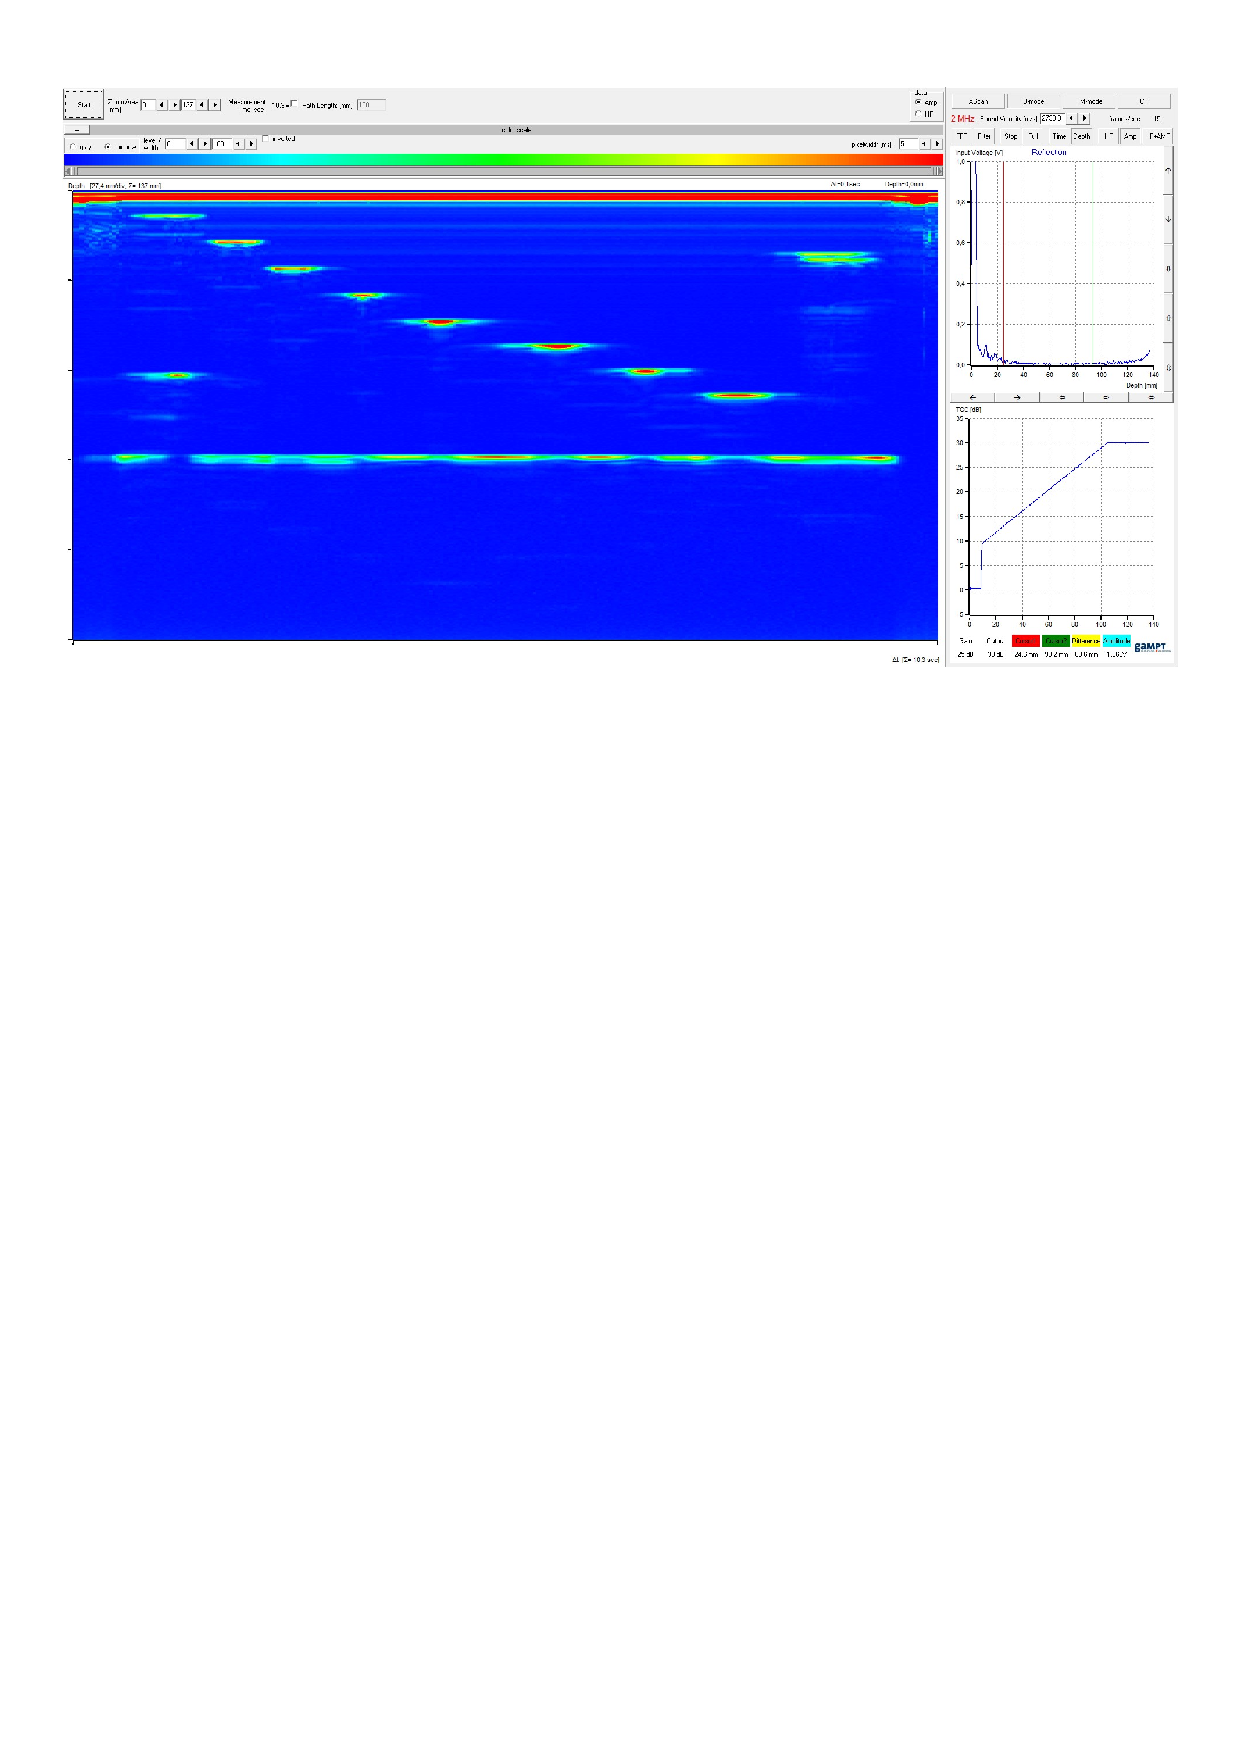
\includegraphics[height = 4cm]{bscan oben.pdf}
    \caption{B-Scan von der Oberseite.}
    \label{fig:boben}
\end{figure}
\begin{figure}
    \centering
    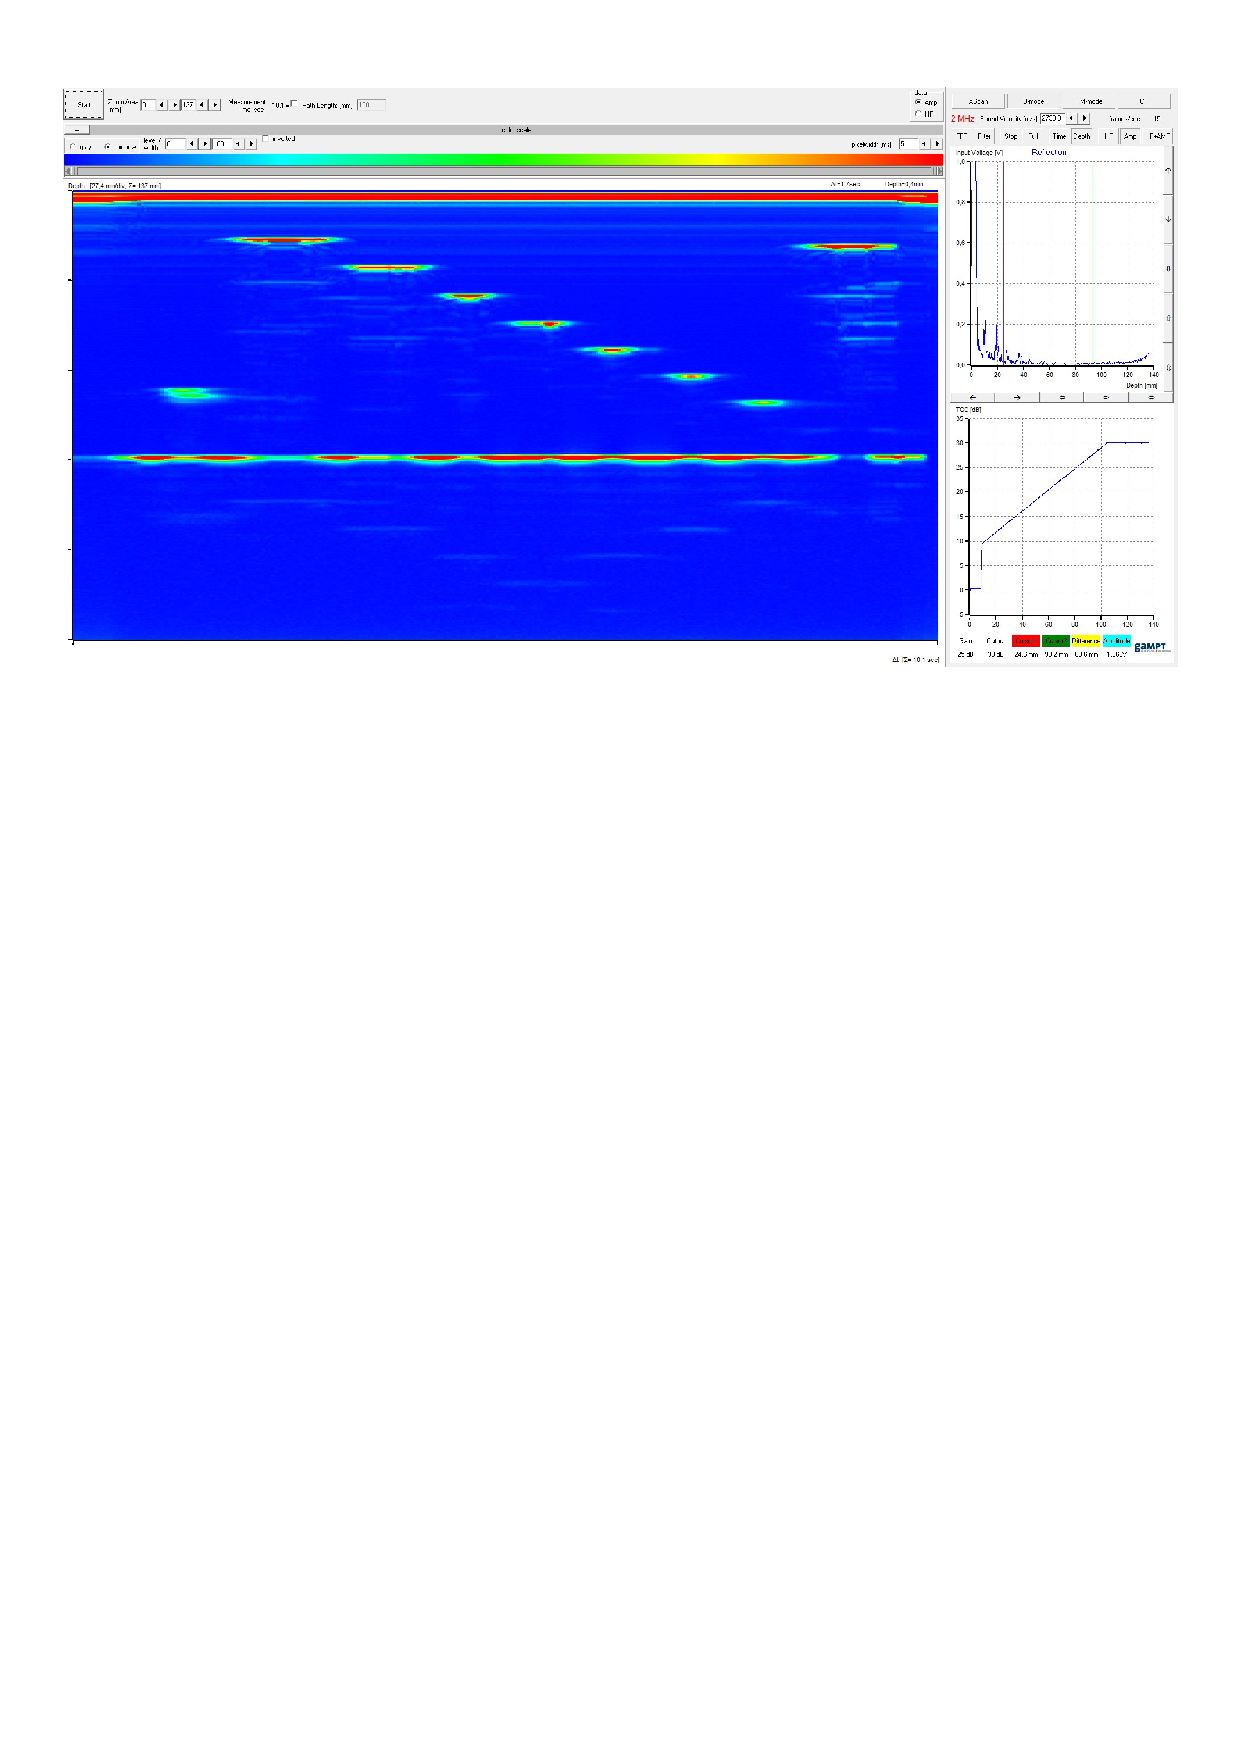
\includegraphics[height = 4cm]{bscan unten.pdf}
    \caption{B-Scan von der Unterseite.}
    \label{fig:bunten}
\end{figure}

\begin{table}
    \centering 
    \caption{Messwerte der Tiefe der einzelnen Bohrungen sowie dessen errechnete Durchmesser.}
\begin{tabular}{c | c c | c c | c}
    \toprule
    & \multicolumn{2}{c}{oben}& \multicolumn{2}{c}{unten} & \\
    Bohrung & Tiefe \/\unit{\mm} &  nach Korrektur \/\unit{\mm}& Tiefe \/ \unit{\mm} & nach Korrektur \/ \unit{\mm} & d \/ \unit{\mm}\\
    \midrule
           1 & 21.1 & 20.0 & 60.8 & 59.7 & 0.2\\
           2 & 19.3 & 18.2 & 62.2 & 61.1 & 0.6\\
           3 & 62.4 & 61.3 & 14.9 & 13.8 & 4.6\\
           4 & 55.1 & 54.0 & 23.6 & 22.5 & 3.4\\
           5 & 47.5 & 46.4 & 31.9 & 30.8 & 2.7\\
           6 & 40.1 & 39.0 & 40.8 & 39.7 & 1.5\\
           7 & 31.9 & 30.8 & 48.7 & 47.6 & 1.5\\
           8 & 23.7 & 22.6 & 56.4 & 55.3 & 2.0\\
           9 & 15.8 & 14.7 & 64.5 & 63.4 & 1.8\\
           10& 8.0  & 6.9  & -- & -- &     \\
           11& 56.2 & 55.1 & 17.2 & 16.1 & 8.7\\
    \bottomrule
    \end{tabular}
    \label{tab:BScan}
\end{table}

\subsection{Lokalisierung und Identifizierung der Tumore.}
\begin{figure}
    \centering
    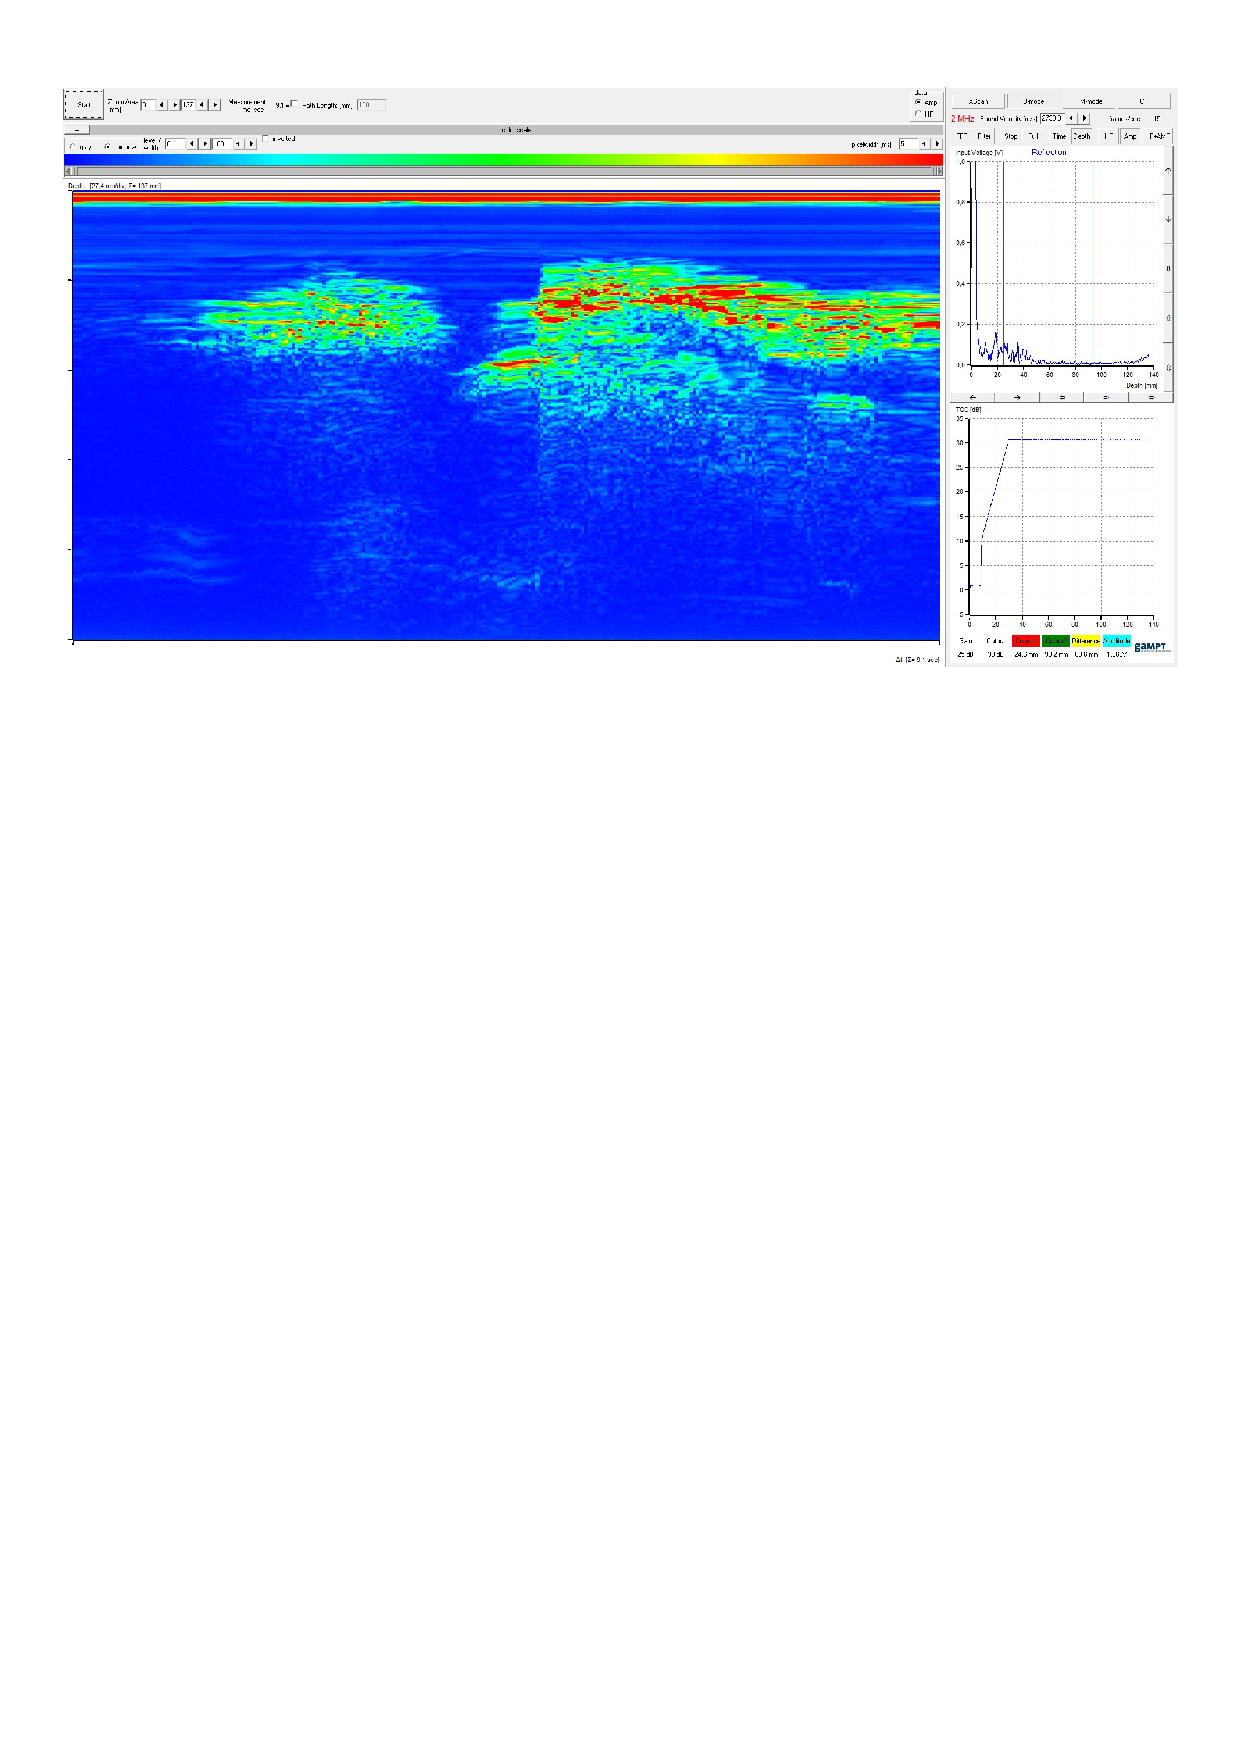
\includegraphics[width = 4cm]{vier.pdf}
    \caption{B-Scan der Tumore.}
    \label{fig:Tumore}
\end{figure}
In \autoref{fig:Tumore} sind die entdeckten Tumore abgebildet. Es ist deutlich zu sehen, dass der rechte sowohl größer als auch dichter als der Linke ist. Aufgrund des unterschiedlichen Aussehens bzw. der
unterschiedlichen Farbgebung lässt sich vermuten, dass es sich bei dem linken Tumor um eine Zyste und beim rechten um ein Tumor aus Gewebe handelt.